\documentclass[openright,11pt,twoside,a4paper]{report}
\usepackage[utf8]{inputenc}
\usepackage{hyperref}
\usepackage{listings}
\usepackage{color}
\usepackage[parfill]{parskip}
\usepackage{tabularx}
\usepackage{array}
\usepackage{url}
\usepackage{comment}
\usepackage{graphicx}
\usepackage{caption}
\usepackage{subcaption}
 
\definecolor{dkgreen}{rgb}{0,0.6,0}
\definecolor{gray}{rgb}{0.5,0.5,0.5}
\definecolor{mauve}{rgb}{0.58,0,0.82}
 
\lstset{ 
  language=Java,                % the language of the code
  basicstyle=\footnotesize,           % the size of the fonts that are used for the code
  numbers=left,                   % where to put the line-numbers
  numberstyle=\tiny\color{gray},  % the style that is used for the line-numbers
  stepnumber=1,                   % the step between two line-numbers. If it's 1, each line 
                                  % will be numbered
  numbersep=5pt,                  % how far the line-numbers are from the code
  backgroundcolor=\color{white},      % choose the background color. You must add \usepackage{color}
  showspaces=false,               % show spaces adding particular underscores
  showstringspaces=false,         % underline spaces within strings
  showtabs=false,                 % show tabs within strings adding particular underscores
  frame=single,                   % adds a frame around the code
  rulecolor=\color{black},        % if not set, the frame-color may be changed on line-breaks within not-black text (e.g. commens (green here))
  tabsize=2,                      % sets default tabsize to 2 spaces
  captionpos=b,                   % sets the caption-position to bottom
  breaklines=true,                % sets automatic line breaking
  breakatwhitespace=false,        % sets if automatic breaks should only happen at whitespace
  title=\lstname,                   % show the filename of files included with \lstinputlisting;
                                  % also try caption instead of title
  keywordstyle=\color{blue},          % keyword style
  commentstyle=\color{dkgreen},       % comment style
  stringstyle=\color{mauve},         % string literal style
}

\usepackage{graphicx}
\graphicspath{{./images/}}

\begin{document}

\begin{titlepage}

\newcommand{\HRule}{\rule{\linewidth}{0.5mm}} % Defines a new command for the horizontal lines, change thickness here

\center % Center everything on the page
 
%----------------------------------------------------------------------------------------
%	HEADING SECTIONS
%----------------------------------------------------------------------------------------

\textsc{\LARGE Norwegian Univeristy of Science and Technology}\\[1.5cm] % Name of your university/college
\textsc{\Large TDT4501}\\[0.5cm] % Major heading such as course name
%\textsc{\large Minor Heading}\\[0.5cm] % Minor heading such as course title

%----------------------------------------------------------------------------------------
%	TITLE SECTION
%----------------------------------------------------------------------------------------

\HRule \\[0.4cm]
{ \huge \bfseries Using motion based game controllers as sensors for a mobile biofeedback system: Technological challenges}\\[0.4cm] % Title of your document
\HRule \\[1.5cm]
 
%----------------------------------------------------------------------------------------
%	AUTHOR SECTION
%----------------------------------------------------------------------------------------

\begin{minipage}{0.4\textwidth}
\begin{flushleft} \large
\emph{Authors:}\\
Dean \textsc{Lozo}\\ % Your name
Knut \textsc{E. M. Nekså}\\ % Your name
\end{flushleft}
\end{minipage}
~
\begin{minipage}{0.4\textwidth}
\begin{flushright} \large
\emph{Advisor:} \\
Dag \textsc{Svanæs} % Supervisor's Name
\end{flushright}
\end{minipage}\\[3cm]

% If you don't want a supervisor, uncomment the two lines below and remove the section above
%\Large \emph{Author:}\\
%John \textsc{Smith}\\[3cm] % Your name



%----------------------------------------------------------------------------------------
%	LOGO SECTION
%----------------------------------------------------------------------------------------


\includegraphics{ntnuEnglish.png}\\[1.5cm] % Include a department/university logo - this will require the graphicx package

%----------------------------------------------------------------------------------------
%	DATE SECTION
%----------------------------------------------------------------------------------------

{\large \today}\\[3cm] % Date, change the \today to a set date if you want to be precise

%----------------------------------------------------------------------------------------

\vfill % Fill the rest of the page with whitespace

\end{titlepage}

\cleardoublepage
\begin{abstract}
An abstract here perhaps?
\end{abstract}

\tableofcontents

\chapter{Introduction}
%The Introduction is your thesis in a nutshell. Again, the organization can vary, but a standard introduction includes the following sections:

\section{Purpose}
The purpose of the project is to explore the possibility of creating a mobile bio-feedback system through the use of a smartphone and cheap mass produced peripherals. The smartphone will act as a hub, while sensor based peripherals attached to the user will gather information. The information will be processed by the smartphone, and appropriate feedback will be provided to the user; Feedback will be provided by using vibration and audio. By acknowledging the feedback the user can improve his or her gait, and reduce the likelihood of a fall.

\section{Motivation}
%Brief description of the research domain and the problem that one wants to address. It should tell the reader why working on this project is worth doing.
Falls are a major health hazard among the elderly population (age > 65) \cite{fallsHealthHazard}, in addition to being an obstacle for physical activity and independent living. Through physical activity the elderly may improve their quality of life and prevent future disabilities\cite{physicalActivity}. A third of all elders that experience a fall develop a fear of falling \cite{fearOfFalling}. Fear of falling causes general anxiety and avoidance of physical activity. Long term consequences result in social isolation, physical deterioration and reduced quality of life.\cite{physicalAvoidance} %Skrive noe om hvor mye det koster staten å passe på de eldre?

Between 30\% and 60\% of the elder population will experience at least one fall per year, and 10\% - 20\% of these will result in an injury, hospitalization or death \cite{fallStatistics}. For the independent elder population it is even more crucial that a fall can be avoided and the proper authorities can be alerted if a fall does occur. In the case of a serious fall a slow response time might increase the likelihood of permanent damage or death\cite{personHomeDeath, dangerousFallHome}.

Technological progress has made it easy and affordable to incorporate sensors into devices in order to provide a better or more entertaining user experience. Accelerometers, gyroscopes and GPS are an expected feature in today's smartphones. Newer phones include even more advanced sensory such as Barometers, and Proximity Sensors.

Motion based games and game controllers have been a trend in the gaming industry for the last 8 years. It started with the Nintendo Wii, but Microsoft Kinect and Playstation Move followed quickly with their own motion detection technology. The competition to offer the best product on the market has made motion sensing more powerful, while mass production has made it cheaper.

\section{Research goals}
%What are the questions you are answering with your project? Normally, you specify a main question and related sub-questions. Remember that at the end you have to demonstrate you have answered to the stated questions. It is not uncommon that the questions are changed during the project, but it is important to be as explicit as possible and as early as possible with research questions since they help you to focus.
The primary research goal is to develop a mobile bio-feedback system through mass produced off the shelf products. A smartphone will function as the central hub for the system. Game controllers with motion detecting capabilities will be attached to the user in key locations and transmit sensor data to the smartphone. The phone will process the data, compute it. The user will control and interact with the system through the smartphone. The system will provide the user with feedback through audio and vibration. In addition to the audio on the phone, a bluetooth speaker can be connected, and the game controllers provide vibration and audio as well.

%PRETTY PICTURE THAT SHOW HOW THINGS WORK TOGHETER IN THE SYSTEM
\begin{figure}[h!]
  \centering
    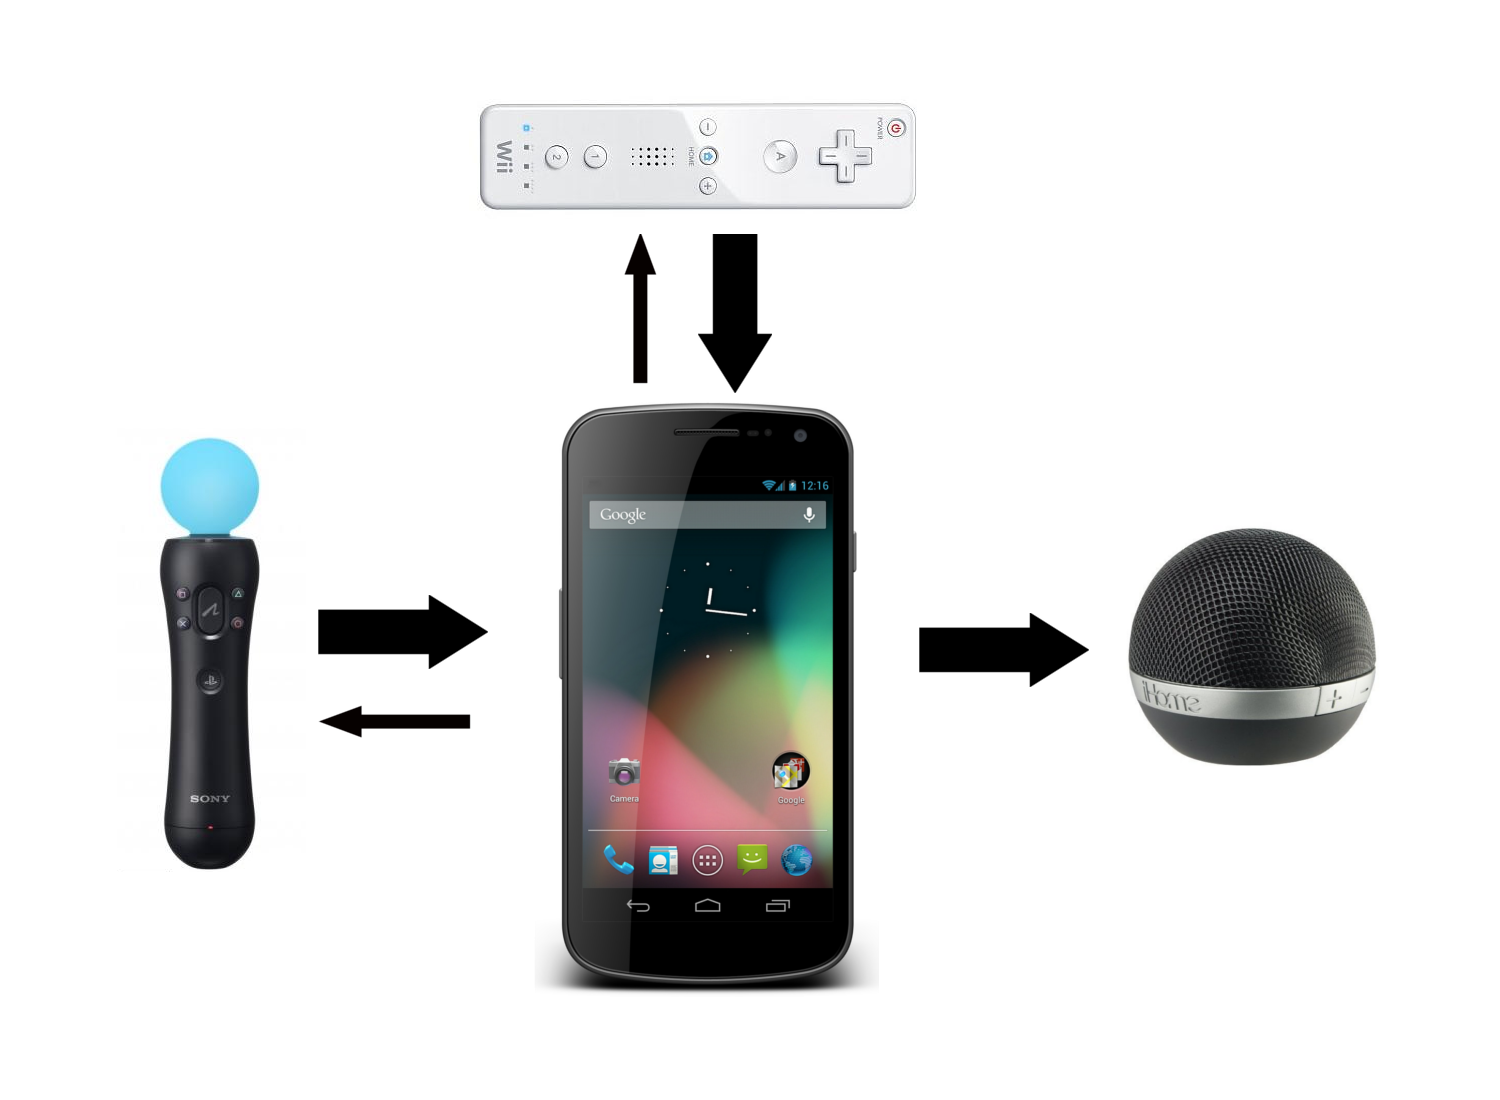
\includegraphics[width=.80\textwidth]{hub.png}
    \caption{\footnotesize A conceptual image of the hardware involved in a mobile bio-feedback system. Arrows represent the information flow, and the thickness represent the intensity.}
\end{figure}

In order to reach the primary goal mentioned above, a set of sub-goals must be completed. The sub goals will help strengthen the viability of the system in an uncontrolled changing environment.

\begin{itemize}

\item Develop a library for Android that can receive a bit stream with sensor data from a gaming peripheral via bluetooth. A Wii Remote with Motion Plus will be the first to be tested and implemented.

\item Develop a basic application that can be distributed on several Android devices. A qualitative test will be preformed in order to confirm that the application is function properly on the device.

\item Perform tests to measure the durability and of the system. Battery life, range and stability are factors that will affect the viability of the system.

\item Conduct a set of small scale tests to see if the system has any potential as a bio-feedback system.

\end{itemize}


\section{Research method}
%How the research is conducted. In the previous section you say what you are doing. Here you specify how. The choice of a research method is strictly connected to the type of questions you want to answer.
This section will provide a brief summary of the research methods that have been considered and relevant papers that present them. The final choice of research method will be presented at the end of the section, with an explanation as to why the method was chosen. Victor R. Basili\cite{paradigm} is the first paper to be looked. He identifies different experimental paradigm in Software engineering. The paper defines two main methods, the scientific method, and the mathematical method. The second paper is a guideline for conducting and reporting a case study in software engineering by Runeson and Höst.


\subsection{The Scientific Method}
The scientific method is based on observing the world, proposing a model or a theory of behaviour, measuring and analyzing and finally validating the hypothesis of the model or theory. If possible the procedure should be repeated. In software engineering this paradigm is suited when trying to understand the software process, product, people and environment. The idea is to extract some form of model that attempts to explain the underlying phenomena and evaluate whether the model is a correct representation of the phenomena being observed. An example might be when trying to understand how an organization develops software to see if a tool can be built to automate parts of the process. There are two variations of this inductive approach.

The engineering method observes existing solutions, proposes better solutions, builds the better solutions, analyzes and measure the new solution, and repeats the process until no further improvements can be made. This approach is an evolutionary improvement oriented approach which assumes one already has models of the product, software process, people and environment and focuses on modifying it in order to improve object of study. An example might be a study of tools used in the development process, and demonstrating how other tools can assist them better in their way of work then the ones they are currently using.A crucial part for this method is the need for careful analysis and measurement.

The empirical method a model is proposed, statistical/qualitative methods are developed, and applied to case studies. It results are analyzed and measured, and then used to validate the model. The procedure should be repeated as to confirm findings if resources and time allow it. This paradigm is a revolutionary improvement oriented approach which begins by proposing a model that is not necessarily based upon an existing one, and atempts to study the effects of the process or product suggested by the new model. Measurment and analysis is crucial to the success of this method. Simply proposing a model or a new tool is not enough. A way to validate that the proposed model or tool is superior to the current solution must be created.

Experiments must be guided, there has to exist a rational for collecting data. The experiment must be designed to collect information suitable for building a model of the system being studied. An underlying framework must exist that will be used to interpret the collected data.

\subsection{The Mathematical Method}
The mathematical method involves proposing a formal theory or set of axioms, develop a theory, derive results and if possible compare with empirical observations. This approach is a deductive analytic model which does not require an experimental design in the statistical sense, but provides an analytic framework for developing models and understanding their boundaries based upon manipulation of the model itself. Treatment of programs as mathematical objects and their analysis of the mathematical object or its relationship to the pgroam satisfies this paradigm.

% %WRITE A GUIDELINE ABOUT CASE STUDIES HERE


There is very little to no research done on connecting smartphones and gaming peripherals together, and a working system that combines the two does not currently exist. Am explorative case study will conducted in order to perform thorough research on any technical possibilities and limitations as a result of the hardware and software choices for the system. The case study seemed as a natural choice when having to create the system from scratch in the span of 3 and a half months.

The case study will be split into two parts. The first part will focus on achieving research goal (a) and (b) through a qualitative study. It will focus on the technical aspect of the goals. Technical possibilities and limitations encountered during implementation will be discussed and reported. The application will be presented in detail where architecture, functionality, and appearance of the prototype will be discussed.

The second part will focus on reaching research goal (c) and (d) through a more quantitative study. A set of tests will be outlined and conducted in order to test the durability of the system. The tests will be limited to a small amount of devices due to resource and time constraints, but several tests will be run in order to acquire reliable data.

\section{State of the Art}
%This chapter provides an overview of the literature. It positions your work with respect to work already done by others. 

Several attempts have been made to create fall detection systems using smart phone technology \cite{iFall, semiSupervisedFallDetection, mobilePhoneBasedFallDetection, detectionOfFalls}, all of these studies show positive results. The current trend shows that smart phones are becoming more affordable \cite{find_some_data_here} and with the correct software these phones can notify healthcare personnel about falls, giving the elderly an extra safety.

Another approach is to try preventing the falls from happening all together by notifying the user that he or she is moving in an unstable manner. Multiple studies show that using biofeedback systems to inform the user about unstable walk helps prevent falls \cite{multiModualBiofeedback, vibrotactileBiofeedback, vibrotactileTiltFeedback}. % KANSKJE SKRIVE NOE OM AT SENSORENE ER DYRE ELLER TUNGVINTE Å BRUKE I HJEMMET?
Also mobile versions of such systems have been researched with promising results \cite{fallPrevention}.

A limitation for many of the previously discussed solutions is that they only make use of the embedded accelerometers in the smart phone. Increasing the number of sensors and their positioning can make the fall detection application more accurate \cite{fallDetectionWithExtraSensors}.

In this study the goal is to examine if using cheap external sensors can give more accurate and additional sensor data to help make fall detection/prevention applications more effective. The sensors examined will be the Wii Remote and the Sony Move controller. These are cheap mass produced game controllers with embedded sensors and Bluetooth support. Using Bluetooth wireless technology the sensors can be connected to the smartphone and stream supplementary acceleromter and gyroscope data.

The Google Play Store has 3 applications that allow a user to connect a WiiRemote to an Android Device. All of these applications focus only on the buttons, and ignore sensor data \cite{wiimoteController, simpleWiiController}. The applications seem unstable and are far from user friendly, but they are the only of its kind out there.


\chapter{Technology and Software}
In this chapter we discuss the technology that will be used to implement our solution. Android, Playstation Move and Wii Remote are described in detail. We also look at existing applications with similar functionality to our own system. 

\section{Android OS}
Android is a Linux based operating system primarily designed for touchscreen devices such as smartphones and tablets. It is developed by Google and is supported by The Open Handset Alliance (OGHA). The source code was released as open source under the Apache License, and The Android Open Source Project is tasked with maintaining and further developing the operating system. The OGHA is a consortium focused on developing open standards for mobile devices, and members of the consortium are not allowed to produce phones that are not compatible with the Android OS. Applications for the Android OS are primarily written in a customized version of Java using the Software Development Kit, but it is possible to partly write applications in C and C++ using the Native Development Kit. 

Given that the Android OS code is open source and highly modifiable both the community and smartphone distributors have taken advantage of this. Smartphone producers such as HTC and Samsung have made their own versions of the Android OS. These versions come preinstalled on the devices and are referred to as stock firmware. The modifications are primarily focused on making the user interface more powerful and user friendly in order to enhance the user experience \cite{htcSense}. The Android community has also developed their own versions of the Android OS. This firmware might be specialized to be lightweight, or allow a high degree of customization. to better suit advanced users. The best known and most complete community firmware is the CyanogenMod \cite{cyanogenMod}. In order to install and use custom firmware a user needs to ``root’’ the phone. Rooting the phone gives the user access to the entire system, allowing the old firmware to be removed and the new community firmware to be installed.

The software center for Android is known as ``Google Play’’ and allows developers to easily distributed their applications. Users can then choose and download thousands of applications, some are free, while others have to be paid for. The idea is that as long as a device runs the Android OS it can run any of the applications on Google Play. The first Android device was sold in October 2008. By the end of 2010 the Android OS had become the leading smartphone platform \cite{androidLeadingPlatform}, and at the second quarter of 2012 it had a worldwide smartphone market share of 68\%\cite{androidMarketShare}. During the third quarter of 2012, 500 million devices had been activated and there are approximately 1.3 million activations per day \cite{androidDevices}. As of writing, the newest Android version is 4.1, codename Jelly Bean. Figure~\ref{fig:verDist} shows how the different versions are distributed on existing Android smartphones. As the figure shows, most devices have not been updated to the latest version, either because of hardware limitations or because the stock firmware has not been updated by the vendor. With each new version of Android the developer API is improved and functionality is added. Applications using a lower API level developed for earlier Android versions can run on higher API levels, but not the other way around. Using a lower level API allows an application to support more devices, but sacrifices added features and optimization located in a higher level API.

\begin{figure}[h!]
  \centering
    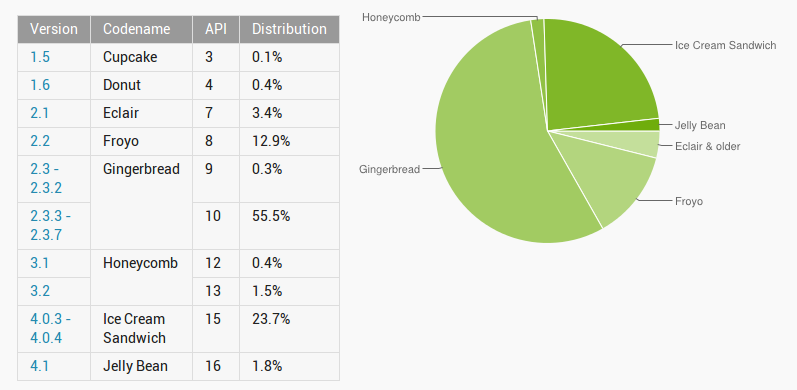
\includegraphics[width=1.0\textwidth]{androidVersionDistribution.png}
    \caption{\footnotesize Version distribution as of October, 2012. The data is based on Android devices that accessed Google Play during a 14 day period \cite{androidVersions}}
  \label{fig:verDist}
\end{figure}

\subsection{Architecture}
Older Android versions are based on Linux kernel 2.6 while Android version 4.0 and higher use Linux kernel 3.0. Google has made alterations to the standard Linux kernel by not including all the standard libraries (see figure~\ref{fig:androidArchitecture})k, this makes porting existing Linux desktop applications difficult. The kernel interacts with the hardware and contains all the necessary drivers in order to do so. As the operating system was designed to run on a variety of hardware, the kernel functions as an abstraction layer between the hardware and software in addition to handling the standard kernel tasks such as resource management, networking and security.

\begin{figure}[!h]
  \centering
    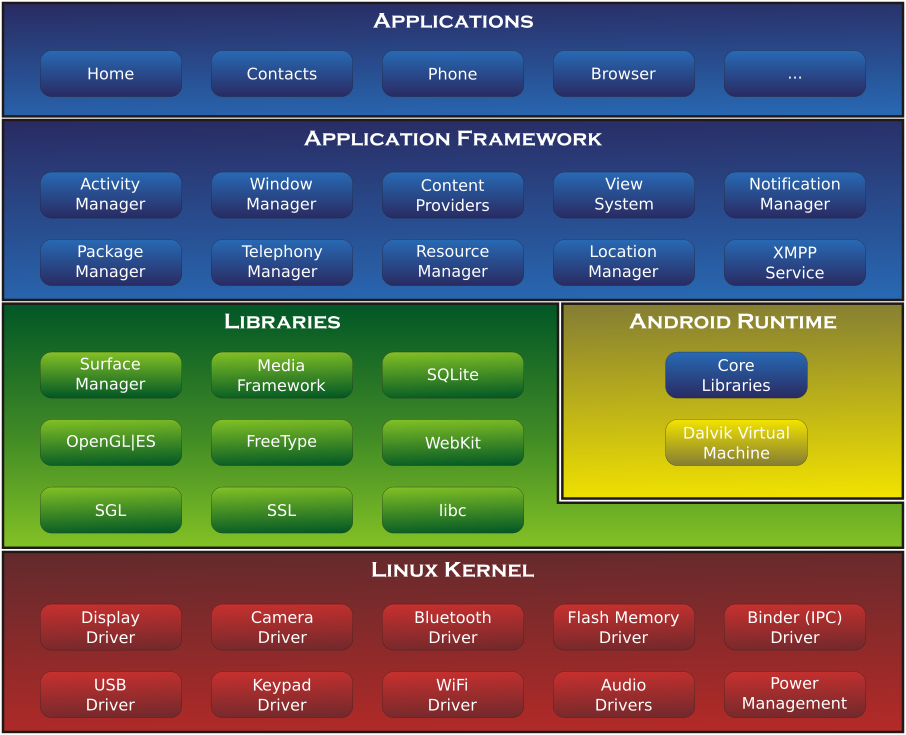
\includegraphics[width=1\textwidth]{androidArchitecture.png}
    \caption{\footnotesize A visual representation of the Android architecture}
 \label{fig:androidArchitecture}
\end{figure}

The library layer contains the native android libraries that enable android devices to handle different types of data. The libraries are written in C++ or C and are hardware specific. These libraries can be accessed through the use of the Android NDK and is recommended for functionality not attainable through the standard SDK. There are dozen of native libraries but some of them include: Webkit is the browser engine used to display HTML content, SQLite is used for data storage locally on the device, OpenGL to render 2D and 3D graphics, in addition to several media codecs. Google has developed their own Java Virtual Machine called the Dalvik Virtual Machine. It runs Android applications and is optimized for low memory and low processing power environments. It provides most of the same features as the JVM such as isolation, multi-threading and memory management. The DVK in addition to core java libraries are called the Android Runtime.

The Application Framework level is what applications on the Android device interact with. Developers use the programs located in this framework as tools to build their own applications. These programs provide access to and manage basic phone functions, such as GPS tracking (Location Manager), sharing data between applications(Content Providers) voice calls (Telephone Manager), applications lifecycles (Activity Manager) and so on. Any application installed by the user is located in the top application layer. These are applications created by developers and can range from SMS clients, to 3D games.

\section{Existing Applications}
The Google Play Store contains a handful of applications that enable an Android device to be connected to a Wii Remote through Bluetooth. The majority of these applications only provide basic features such as key presses, led lights, and rumbling \cite{wiimoteController, simpleWiiController}. There was one application that stood out and utilized the motion detection features of the Wii Remote and gave the sense of a complete application. Wii Motion Monitor \cite{wiiMotionMonitor} turns the Wii MotionPlus into a motion sensor, and is able to represent the orientation of the Wii Remote correctly. Yaw was off by about 45 degrees, but pitch and roll worked perfectly. This proves that the Wii Remote can be used for motion detection and an Android device can act as a hub.

There was only one application \cite{sixaxisController} that enabled a user to connect a SixAxis Playstation 3 controller to an Android device. The application requires root access, and additional work had to be done before the controller was ready to be paired. A compatibility checker is available to see if an Android device is compatible with the software.

\section{Playstation Move}
This section looks closer at the Playstation Move controller. First we will look at the hardware and relevant sensors that we can utilize. Second we will look at relevant libraries that can be used to establish a connection to the controller.

\subsection{Motion Controller Hardware}
The PS Move motion controller contains advanced motion sensing, making it an ideal peripheral for a biofeedback system. It features three different types of sensors: accelerometer, gyroscope and magnetometer. Accelerometer and gyroscope is used for motion tracking, and the magnetometer provides the horizontal orientation based on the earth’s magnetic field. The built in vibration and orb light can be used to provide feedback to the user \cite{psMoveTech}. Unlike the Wii Remote it uses built-in batteries that can be charged using a USB-mini cord. 

\subsection{PS Move API}
The PS Move API \cite{PSMoveAPI} is written in C, but contains bindings for various languages, including Java and C\#. Both of these languages are used in smartphone application development. The API explicitly mentions that it runs on Android devices.This is only partially true: It will not run out of the box on an Android device, restructuring and heavy modification of the Android device is required. The Android OS runs on top of a modified Linux kernel, this kernel does not contain the necessary libraries and drivers in order for the API and Motion controller connectivity to function properly. The next step would be to compile the C API into a shared library using the Android NDK, and use the shared library Java bindings in the Android Java code. The lead developer has implemented a working application on a smartphone with a custom kernel, but states that due to the Android kernel he is having a hard time making it work ``out of the box’’ and is only a proof of concept. The API is still in development as of writing.

Because of the technical challenges and the lack of documentation on the reverse engineering of the Playstation Move, it was decided that the Wii Remote was a better choice for the controller. If the API was more mature, and the Android kernel had more drivers it would have been viable. An alternative approach would be to use a smartphone running Ubuntu, which is currently under development \cite{ubuntuAndroid}.

\section{Wii Remote with MotionPlus}
In this section we present the Wii Remote and MotionPlus hardware, and describe some of the third-party libraries that exist for connecting to the device.

\subsection{Wii Remote and Motion Plus Hardware}
The original Wii Remote features motion tracking for vertical movement, left-right horizontal movement, and horizontal rotation through the use of an ADXL330 accelerometer.\cite{wiiAccelerometer}. In June 2009 Nintendo released the Wii MotionPlus expansion device which contains a dual-axis tuning fork and a single-axis gyroscope\cite{wiiMotionPlus}. The expansion device improves the motion tracking of the Wii Remote greatly, but makes it larger. Nintendo has now started selling the Wii Remote Plus. It is the same size as the Wii Remote, but has the Wii MotionPlus already built in. Both of the controller types have the ability to provide vibration and basic audio feedback.

\subsection{Wii Remote API}
At the time of writing no open source Wii Remote library has been published for the Android OS. Though some Wii Remote libraries exist, none of them are intended to be used on Android devices. The next subsections will cover the libraries that are implemented in Java.

\subsubsection{WiiRemoteJ}
WiiRemoteJ is one of the most complete libraries for the Wii remote. It is a pure Java library with support for a large amount of Wii extensions such as the Wii Guitar, and Wii Balance Board. It does however lack support for the MotionPlus extension. The library has not been update since July 2008. The author has taken down the homepage where the library was originally located, but it can be found on third party websites. \cite{WiiRemoteJ}

\subsubsection{WiiuseJ}
WiiUseJ is a lightweight Java API. It was built on top of the Wiiuse API and only supports the Wii Remote and the Nunchuck. Like the previous library it lacks support for the MotionPlus extension. The project has been discontinued since January 2009. \cite{Wiiusej}

\subsubsection{Motej}
Motej is an open source (licensed under ASL 2.0) library for the Wii remote written in Java. Motej supports only the Wii Remote and IR Camera in its basic form. An extension library exists, adding support for the balance board, classic controller, and nunchuk. The project is currently at version 0.9, and was discontinued in 2009. \cite{Motej}

\section{Bluetooth}
Bluetooth is a short-range communication technology that is simple and secure. The technology aims to provide a wireless alternative to cables when connecting two devices. Key features such as robustness, low cost, and low power consumption has made it one of the leading standards in its field and is supported by most modern operating systems through integrated hardware or portable Bluetooth adapters.

When a secure connection is established between two Bluetooth devices it is referred to as pairing. The devices can then securely communicate and transfer data with each other. Bluetooth is based on a master-slave architecture, allowing a single device to have up to 7 slaves, meaning that package exchanges are based on the masters clock. This is known as a piconet and a device can be a member of several piconets simultaneously. Bluetooth has three different classes of radios. The class specifies the range and power consumption of the radio. Most devices, including mobile phones and game controllers, use the Class 2 radio. Class 2 allows a range of at least 10 meters and consumes 2.5mW of power \cite{bluetooth}.

Bluetooth comes with different stacks of protocols. In Bluetooth devices designed for smartphones use the Radio Frequency Communications (RFCOMM) protocol. RFCOMM is based on the lower level Logical Link Control and Adaptation Protocol (L2CAP), and provides a reliable data stream with serial port emulation. Both Playstation Move and Wii Remote uses the L2CAP for communication. This low level protocol is not directly supported by the current version of Android, how we solved this issue is described further in the section~\ref{sec:motejOnAndroid}.
\chapter{Prototyping}
%Development
Since no library with Android support currently exist it was decided to use the Motej library as a core for further development.

\section{Introduction}
At the time of writing no research has been done on using motion game controllers as peripherals in a smart-phone based bio-feedback system. In order to answer the research questions posed in this report it will be necessary to create a simple but working prototype of the aforementioned system. The equipment used to realize the system will be a rooted HTC Desire HD \cite{desireHdSpecs} running CyanogenMod 7 and Wii Remotes with the Motion Plus extension. The application will be created using the Android SDK, Java and the Motej library.
%Write about why we chose motej?

\section{Wii remote reverse engineering}
This section will look closer on the reverse engineering of the Wii remote. Since the Wii remote is the only sensor to be used in this project, it is important to explain in detail how the data from this sensor is parsed and calibrated. In this section there will be multiple references to Motea. Motea is a lightweight Wii remote API based on Motej \cite{Motej}, designed specially for this project. A further description of Motea can be found in section~\ref{sec:motea}

Nintendo has not released any documentation of how to connect to or use the Wii remote. All the information in this section is taken from internet communities \cite{wiiBrew} that have reverse engineered the Wii remote and from open source Wii remote API projects \cite{wiiMoteLib, Motej}.

The Wii remote is based on the HID protocol for communication, and will appear as such to any host. It is possible to connect to the Wii remote both with and without Bluetooth pairing. If paired the Wii remote will attempt to reconnect to the host if the connection is lost. In the current version Motea no pairing is performed. A HID connection is established using L2CAP, opening a data channel on port 0x13. This channel is used for both sending and receiving data.

\subsection{HID interface}
The different report types used in the Motea library are displayed in table~\ref{tab:hidInterface}. An output report represents a report that is sent from the host to the Wii remote. An input report is a report that is sent from the Wii remote to the host. Input reports are prefixed with 0xa1 and output reports are prefixed with 0xA2.There are more input reports than those listed in table~\ref{tab:hidInterface}, but they are not used by Motea since data report 0x35 contains all the data needed. 

\begin{table}[h!]
\centering
\begin{tabularx}{\textwidth}{|l|l|X|}
\hline
I/O & ID & Description \\ \hline
O & 0x11 & Set LEDs \\ \hline
O & 0x12 & Set data reporting mode \\ \hline
O & 0x15 & Request status information \\ \hline
O & 0x16 & Write to memory/registers \\ \hline
O & 0x17 & Read from memory/registers \\ \hline
I & 0x20 & Status information \\ \hline
I & 0x21 & Data from memory/register request \\ \hline
I & 0x35 & Data report containing data from core buttons, accelerometer and extension (gyroscope) \\ \hline
\end{tabularx}
\caption{\footnotesize The table describes the different output and input reports used by the application}
\label{tab:hidInterface}
\end{table}

\subsection{Output reports}
Motea sets the report mode to 0x35 as soon as the connection to the Wii remote is established. This is done by sending the following bytes to the Wii remote:
\begin{quote}
0xA2 0x12 0x04 0x35
\end{quote}
The first byte indicates that it is an output report, the second byte is the ID of the report type, the third byte indicates whether to use continuous reporting (send report even when there has been no change to the data) and the fourth indicates which report mode to set. The report mode has to be set again whenever an extension is discovered, this can be detected by the fact that you receive a status information report without requesting one. In such cases Motea immediately sends a request to set the report mode to 0x35.

Report mode 0x35 contains core button (0xbb), acceleromter (0xaa), and extension data (0xee):
\begin{quote}
0xA1 0x35 0xbb 0xbb 0xaa 0xaa 0xaa 0xee 0xee 0xee 0xee ... (16 bytes of type 0xee)
\end{quote}

The LEDs on the Wii remote can be controlled by using output report 0x11:
\begin{quote}
0xA2 0x11 0x80
\end{quote}
The third byte indicates which lights to turn on, the four most significant bits of this byte each represents one LED (in the example above the rightmost byte is enabled):
\begin{quote}
0b0000 0000 : no lights\\
0b1000 0000 : rightmost LED enabled\\
0b1100 0000 : the two rightmost LEDs enabled\\
etc.
\end{quote}
Motea also uses this report mode to initialize the rumble pack. The least significant bit of the third byte of any output report turns sets the status of the rumble pack, where 1 is on and 0 is off. As an example, let us say we have the two rightmost LEDs activated and the rumble pack is to be turned on, the report would look like this:
\begin{quote}	
0xA2 0x11 0xC1\\
(0xC1 = 0b1100 0001 the least significant bit representing the rumble pack)
\end{quote}
As previously stated all output reports have to change the least significant bit of the third byte to one if the rumble pack is to stay active. Therefore Motea has to keep track of the state of the rumble pack and change the output reports accordingly. All examples in this section, other than the one above, will assume that rumbling is turned off.

Status information can be requested by sending:
\begin{quote}
0xA2 0x15 0x00
\end{quote}
A status information report with ID 0x20 is then sent from the Wii remote to the host:
\begin{quote}
0xA1 0x20 0xbb 0xbb 0xss 0x00 0x00 0xll
\end{quote}
0xbb (bytes 3 and 4) contains data about the core buttons. 0xss contains data about which LEDs are enabled and whether the following features are enabled: speaker, extension controller, and continouous reporting. 0xll holds the battery level. 

Writing to registers is done by sending:
\begin{quote}
0xA2 0x16 0x04 0xaa 0xaa 0xaa 0xll 0xdd 0xdd ...
\end{quote}
Here 0xaa (bytes 4-6) represents the register address to write to. 0xll is the number of bytes to write. 0xdd (bytes 8-) is the data to be written to the register, usually only one byte is written.

Reading from registers/memory is done by sending:
\begin{quote}
0xA2 0x17 0xmm 0xaa 0xaa 0xaa 0xll 0xll
\end{quote}
0xmm sets whether to read from memory or from the registers, in motea only the calibration report for the accelerometer is read from memory. 0xaa (bytes 4-6) is the address to read from. 0xll (bytes 7 and 8) is the length of data to be read. After a read request is sendt the Wii remote sends the data in return using a report with ID 0x21:
\begin{quote}
0xA1 0x21 0xbb 0xbb 0xse 0xaa 0xaa 0xdd 0xdd ... (16 bytes of the type 0xdd)
\end{quote}
0xb (byte 3-4) is core button data. 0xse holds both the size of the data returned and the error flag. 0xdd (bytes 8-23) contain the requested data (as long as there was no error).

\subsection{Accelerometer}
Accelerometer data is received with every data report of ID 0x35:
\begin{quote}
0xA1 0x35 0xbb 0xbb 0xxx 0xyy 0xzz 0xee 0xee ...
\end{quote}
The accelerometer data each consists of 10 bits of x-axis data, and 9 bits of y- and z-axis data. Y- and z-axis data should also be represented as 10 bits, this is done by always letting the least significant bit be 0 for these axes (0bxx xxxx xxx0 where x is some data). The most significant bits of x-, y- and z-axis accelerometer data are located in 0xxx, 0xyy and 0xzz respectively. The least significant bits are located in he 0xbb bytes as shown in figure~\ref{fig:accelerometerData}, these bytes also contain core button data.
\begin{figure}[h!]
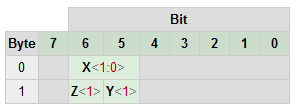
\includegraphics{accelerometerData.png}
\caption{\footnotesize Least significant bits of accelerometer data}
\label{fig:accelerometerData}
\end{figure}

In order to make sense of the accelerometer data they have to be calibrated. The calibration data is stored in the Wii remote and can be acquired by sending a read request:
\begin{quote}
0xA2 0x17 0x00 0x00 0x00 0x20 0x00 0x0a
\end{quote}

The Motej \cite{Motej} library did not contain any code for calibrating the acceleromter data. In Motea the calibration is based on an implementation found in the WiiMoteLib \cite{wiiMoteLib} library. Motea parsing and calibrating accelerometer data:
\begin{lstlisting}
// Get raw data
float x = 
	((bytes[4] & 0xff) << 2) | ((bytes[2] & 0xff) >> 5 & 0x03);
float y = 
	((bytes[5] & 0xff) << 2) | ((bytes[3] & 0xff) >> 5 & 0x02);
float z = 
	((bytes[6] & 0xff) << 2) | ((bytes[3] & 0xff) >> 5 & 0x02);

CalibrationDataReport c = source.getCalibrationDataReport();
if (c == null) {
	return;
}

// Calculate calibrated accelerometer data
x = (float) ((x - c.getZeroX()) / 
	(c.getGravityX() - c.getZeroX()));
y = (float) ((y - c.getZeroY()) / 
	(c.getGravityY() - c.getZeroY()));
z = (float) ((z - c.getZeroZ())	/ 
	(c.getGravityZ() - c.getZeroZ()));

source.fireAccelerometerEvent(x, y, z);
\end{lstlisting}

\subsection{MotionPlus}
\label{sec:gyroParse}
When you plug in a normal extension to the Wii remote it is automatically receive a status information report notifying that an extension has been connected. Pluging in the MotionPlus however, will not result in such a status information report. To check if the MotionPlus extension is pluged in, the two bytes from Wii remote register address 0xA600FE has to be read by sending the read request:
\begin{quote}
0xA2 0x17 0x04 0xA6 0x00 0xFE 0x00 0x02
\end{quote}
After sending this request a data report with ID 0x21 is sent in return containing the requested data. The received data report contains the two bytes read from register 0xA600FE. The meaning of these bytes are shown in table~\ref{tab:motionPlusStatus}. If the MotionPlus extension is not connected the data report will fail with error 7.
\begin{table}[h!]
\begin{tabularx}{\textwidth}{|l|X|}
\hline
Value  & Meaning \\ \hline
0x0005 & MotionPlus is pluged in, but not initialized \\ \hline
0x0405 & No longer active MotionPlus\\ 
\hline
\end{tabularx}
\caption{\footnotesize MotionPlus status}
\label{tab:motionPlusStatus}
\end{table}

After confirming that the MotionPlus extension is pluged in, the next thing to do is to initialize it. This is done by writing 0x55 to 0xA600F0, by sending the following report:
\begin{quote}
0xA2 0x16 0x04 0xA6 0x00 0xF0 0x01 0x55
\end{quote}

When the MotionPlus has been initialized it has to be activated before we can receive data from it. This is done by writing 0x04 to register address 0xA6 0x00 0xFE:
\begin{quote}
0xA2 0x16 0x04 0xA6 0x00 0xFE 0x01 0x04
\end{quote}
After the MotionPlus extension has been activated the Wii remote will send a status information report, informing that an extension has been connected. Now the extension bytes of data report 0x35 will contain gyroscope data form the MotionPlus.

The 32 bytes from register 0xA60020 holds the calibration data for the MotionPlus. According to the WiiBrew wiki \cite{wiiBrew} it is still unclear how they work. However, by looking at the WiiMoteLib \cite{wiiMoteLib} library an implementation using this calibration data was found. Unfortunately this implementation is not very accurate, at least not compared to manual calibration. Aquireing the data is done by sending the read request:
\begin{quote}
0xA2 0x17 0x04 0xA6 0x00 0x20 0x00 0x32
\end{quote}

Extension data is received with every report of ID 0x35:
\begin{quote}
0xA1 0x35 0xbb 0xbb 0xaa 0xaa 0xaa 0xee 0xee 0xee 0xee ... (16 bytes of type 0xee)
\end{quote}
Here 0xbb represents core button data and 0xaa represents acceleration data. The extension data is contained in the 16 last bytes shown by 0xee above. The gyroscope data is contained in the 6 first bytes of the extension data. The data format is shown in figure~\ref{fig:motionPlusDataFormat}. The gyroscope has two modes: fast and slow. These values tells us what type of scaling to use to get the correct degrees per second. According to WiiBrew \cite{wiiBrew} 20 units correspond to 1.45 deg/s in slow mode and 6.59 deg/s in fast mode. Motea uses slightly different values, taken from WiiMoteLib \cite{wiiMoteLib}: 20 units corresponding to 1 deg/s in slow mode and 5 deg/s in fast mode. Which of these values give more accurate data has not been tested, and since the Madgwick algorithm \cite{madgwick} compensates roll and pitch using the acceleromter, a small error in the gyroscope data can be tolerated. 
\begin{figure}[h!]
  \centering
    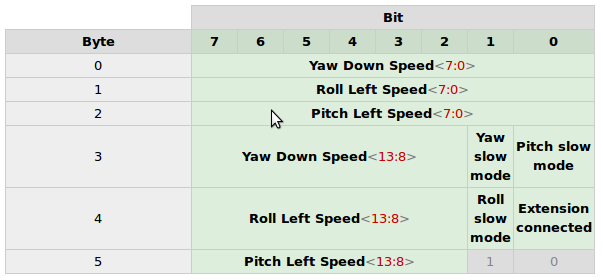
\includegraphics[width=.80\textwidth]{motionPlusDataFormat.png}
    \caption{\footnotesize Motion Plus data gyroscope data format}
    \label{fig:motionPlusDataFormat}
\end{figure}

Motea parsing and calibrating gyroscope data:
\begin{lstlisting}
// Get fast/slow mode
boolean yawFast = ((extensionData[3] & 0x02) >> 1) == 0;
boolean rollFast = ((extensionData[4] & 0x02) >> 1) == 0;
boolean pitchFast = ((extensionData[3] & 0x01) >> 0) == 0;

// Get raw data
float yaw = 
	((extensionData[0] & 0xff) | ((extensionData[3] & 0xfc) << 6));
float roll = 
	((extensionData[1] & 0xff) | ((extensionData[4] & 0xfc) << 6));
float pitch = 
	((extensionData[2] & 0xff) | ((extensionData[5] & 0xfc) << 6));

// Manual calibration
if (!calibration.isFinished()) {
	calibration.addCalibrationData(yaw, roll, pitch);
	if (calibration.isFinished()) {
		calibrationData = calibration.getCalibratedData();
	}
}

// Calibrate raw data
yaw -= calibrationData.getYaw0();
roll -= calibrationData.getRoll0();
pitch -= calibrationData.getPitch0();

// Set scaling
if (yawFast) {
	yaw /= HIGHSPEED_SCALING;
} else {
	yaw /= LOWSPEED_SCALING;
}

if (rollFast) {
	roll /= HIGHSPEED_SCALING;
} else {
	roll /= LOWSPEED_SCALING;
}

if (pitchFast) {
	pitch /= HIGHSPEED_SCALING;
} else {
	pitch /= LOWSPEED_SCALING;
}
\end{lstlisting}

\section{Software Architecture}
In this section contains an explanation and documentation of the various software architectural choices.

The two main focuses when creating the architecture was \emph{modifiability} and \emph{usability}. Modifiability was important to insure the ability to replace the Wii remote with other senors without major changes in the source code. Though the main goal of this project does not include the creation of a complex graphical user interface, usability was still considered a priority for the source code to be reused in future work. 

\subsection{Architectural Patterns}
\subsubsection{Event-driven architecture}
Event-driven architecture is an architectural pattern that focuses on the creation and consumption of events. The event emitters creates new events and pushes them to the event consumers. The event consumers uses the events to produce some reaction. Because the event emitter does not directly speak with the event consumers this pattern makes the different components very loosely coupled.

In our case the event emitters will be the motej and motejx libraries. These classes will handle the connection to the Wii remote and the MotionPlus extension and create events when it receives new date from the Wii remote or its extensions. The event consumers will be the models that change the state in accordance to the received events containing the sensor data. Using this pattern the models are not concerned with the way the event emitters are implemented or what kind of sensors they connect to as long as the events emitted are on the same form.

Fortunatly Motej already implemented the event-driven architecture so there was no need to modify the library in this aspect.

\begin{lstlisting}
//Example of event-driven architecture using 
//java.swing.event.EventListenerList and 
//java.util.EventListener

//Event emittor (parts from the Mote class)
EventListenerList listenerList = new EventListenerList();
...
public void addAcceleromterListener(AcceleromterListener<Mote> listener) {
	listenerList.add(AccelertomerListener.class, listener);
}
...
protected void fireAccelerometerEvent(float x, float y, float z) {
	AccelerometerListener<Mote>[] listeners = listenerList
			.getListeners(AccelerometerListener.class);
	AccelerometerEvent<Mote> evt = 
		new AccelerometerEvent<Mote>(this, x, y, z);
	for (AccelerometerListener<Mote> l : listeners) {
		l.accelerometerChanged(evt);
	}
}

//Interface for the listeners (event consumers)
public interface AccelerometerListener<T> extends EventListener {

	public void accelerometerChanged(AccelerometerEvent<T> evt);

}

//Event consumer - example
public class Example implements AccelerometerListener<Mote> {
	...
	public void acceleromterChanged(AcceleromterEvent<Mote> evt){
		//Events are consumed and handled here
	}
}
\end{lstlisting}

\subsubsection{Model View Controller}
In the model view controller pattern the code is separated into three main components (see figure~\ref{fig:mvc}): model, view and controller. The view handles the graphical user interface and its logic displaying the model to the user. The controller updates the model. The model holds the information or state of the application, which is displayed to the user through the model. This setup gives the users the mental model that they are interacting with the model directly.

\begin{figure}[h!]
  \centering
    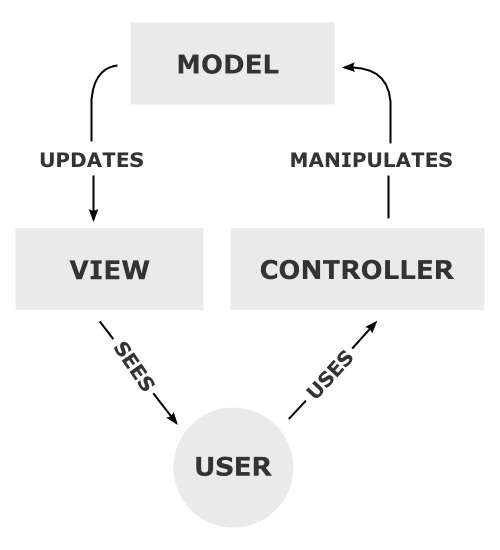
\includegraphics[width=.80\textwidth]{mvc.png}
    \caption{\footnotesize Model-View-Controller pattern}
    \label{fig:mvc}
\end{figure}

Using the model view controller pattern we can easily change the look and feel of the graphical user interface without interfering with how the model is updated. This gives a lot of freedom to continuously modify and improve the graphical user interface during the development of the application. 

\subsection{Package structure}
Using the discussed patterns as a basis, the following package diagram shown in figure~\ref{fig:packageDiagram}. 

\begin{figure}[h!]
  \centering
    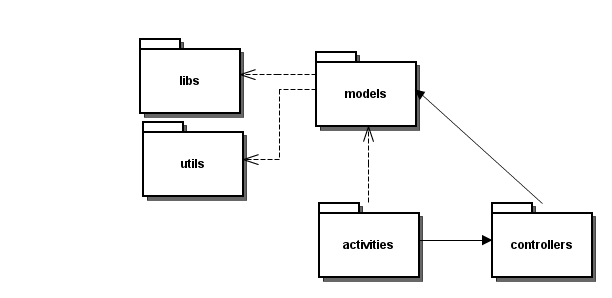
\includegraphics[width=.80\textwidth]{packageDiagram.png}
    \caption{\footnotesize Package diagram}
    \label{fig:packageDiagram}
\end{figure}

\begin{description}
	\item[libs] Contains the library classes used by the project. Currently only contains the java.swing.event.EventListenerList, which is used by Motea. This class is not included in the standard android packages because swing is not part of android.
	\item[utils] The modified Motej library (Modea), our implementation of the MadgwickAHRS algorithm resides here. Motea generates sensor events, and the MadgwickAHRS algorithm is used to calculate orientation.
	\item[models] Classes holding the state of the Wii remote are contained here.
	\item[activities] Holds the Android activity classes. The MainActivity class starts the application and handles Android activity events. The CubeView class is used to generate a 3D-model illustrating the orientation of the connected Wii remote.
	\item[controller] Contains controller classes for interacting with the models and the Wii remote.
\end{description}

\subsection{Activity diagram}
The current application was created to be a proof of concept for the use of Wii remotes in fall detection/prevention applications. Figure~\ref{fig:activityDiagram} displays the basic functionality implemented in the solution. In addition to the 3D model that graphically displays the orientation of the Wii remote, an alarm system was also implemented. This alarm system is activated when the Wii remotes angle is greater than some predefined threshold. This threshold, is as of now, not customizable from the application itself but is hard-coded  into the application for now. 

The alarm uses sound and vibration to notify the user that the Wii remote angle has broken the threshold. Both sound and vibration is given in pulses with a delay between them, as the Wii remote angle becomes grater the delay between each pulse decreases. For the vibrotactile feedback the Wii remote's rumblepack is used and the sound is generated by the Android smartphone speaker. 


\begin{figure}[h!]
  \centering
    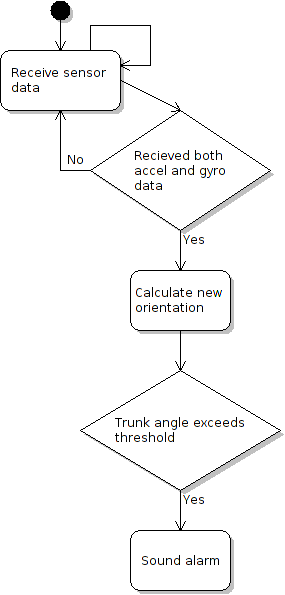
\includegraphics[width=.40\textwidth]{activityDiagram.png}
    \caption{\footnotesize Package diagram}
    \label{fig:activityDiagram}
\end{figure}

\subsection{Class diagram}
Figure~\ref{fig:classDiagram} shows a class diagram of the application's most important classes. The different background colors represents different parts of the system.

The classes with the red background handles the connection to the Wii remote. When the MainActivity class receives a BluetoothDevice object, that object is used to create an instance of Mote. The Mote class connects to the Wii remote. Each second the CheckStatus class is run to get an update about the Wii remote's battery life as well as trying to connect to the MotionPlus, if it is not already connected. The MotionPlus parses the extension bytes received from the Wii remote, it also handles the manual calibration of the gyroscope.

The green background contains the controller classes. WiiMoteHandler handles all communication with the Motea classes (red background). It listens to both the accelerometer and gyroscope events from the Mote instance. When both an acceleromter event and a gyroscope event has been received the WiiMoteHandler WiiRemoteHandlerfires a sensor events. WiiMoteHandler also listens to alarm events to start the rumble pack in the Wii remote when the alarm goes off. Since this class is the only one talking to the Motea classes, this is the only class that needs major changes if it is decided to replace the Wii remotes with other types of sensors. 

AngleCalc listens to sensor events from the WiiMoteHandler, the gyroscope and acceleromter data are used to compute the orientation of the Wii remote and the trunk that it is strapped to. To compute the orientation AngleCalc uses Madgwick's altitude and heading reference system algorithm, which is implemented in the MadgwickAHRS class. AngleCalc then updates the OrientationModel with the newly calculated orientation.

The yellow zone holds the models. OrientationModel hods the current orientation of the Wii remote and then fires an event when it is changed. A very simple noise cancelling system has also been implemented here, to reduce the yaw drift when the Wii remote was kept still. Since the yaw rotation is will not be in the actual fall detection/prevention, this functionality is mainly to make the 3d cube model look better.

ThresholdAlarm listens to orientation events fired by the OrientationModel and then calculates whether the angle of is great enough to fire an alarm event. Alarm events have a severity variable that indicates how great the angle is. In the current implementation this variable is used to reduce the delay between rumble pulses and sound beeps, the greater the angle the faster the beeps.

The views have a blue background. MainAcitivty is the class that starts the application. It also handles Bluetooth discovery and initiates the appropriate classes when a Wii remote is detected. CubeView listens to the orientation evnets from the OrientationModel to crate a graphical representation of the position of the Wii remote. AlarmSound handles playing beeps from the smartphone when the ThresholdAlarm fires alarm events. 

\begin{figure}[h!]
	\centering
	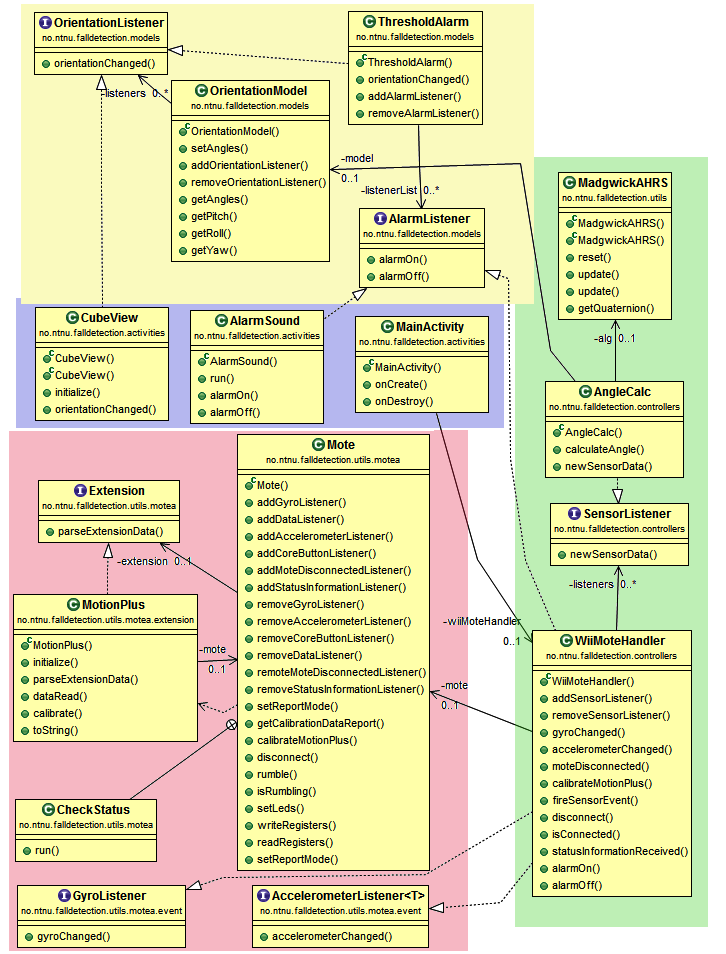
\includegraphics[width=1\textwidth]{classDiagram.png}
	\caption{\footnotesize Class diagram}
	\label{fig:classDiagram}
\end{figure}

\section{Limitations}
%Se på dette avsnittet knut. Tror hele må skriver på nytt hvor avsnittene under er merget og forklart bedre
The majority of Android devices have built-in Bluetooth cards, but the current Android SDK does not offer low level support for the Bluetooth stack, including L2CAP. This constraint can be bypassed on some devices by using reflection to access the socket constructor\cite{l2capHtc}. Access could also be gained through using the Android NDK (Native Developer Kit) but this is outside the scope of this project. Due to L2CAP not being official supported, certain vendors of Android devices have removed the L2CAP protocols completely, meaning that it would be impossible to use their Android OS to connect to the Wii Remote. %Write it more technical
Therefore the Android OS on the HTC Desire HD was altered to run with CyanogenMod 7 instead of the default HTC Sense.

We are unable to connect to new WiiRemote probably due to a different way of initilization.

Have to remove/add the gyroscope in order for the application to register it


\section{Motej and Motejx}
The most complete of the Java based Wii remote libraries that could be found was Motej. Work on the library was discontinued in 2009, but supports all the main Wii remote functionality, and most of the extensions. It was therefore decided to use Motej as the base for a Wii remote library for Android. 

Figure~\ref{fig:motejClassDiagram} shows the most important classes of the Motej and Motejx libraries. To use the library you would create an instance of the Mote object, which takes care of handling the connection to the Wii remote. The Mote constructor takes a string with the bluetooth address of the Wii remote to connect to as input. It is also possible to use the MoteFinder class to discover any Wii remotes that are broadcasting for a connection. The Motej instance fires events whenever it receives data from the Wii remote, these events can be listened to by implementing the different listeners in the motej.events package. 

Wii remote extensions are handled by the Motejx library, which is an extension to the Motej library. All supported extensions have to be added to a extensions.properties file, which contains the extension id and the class that handles that type of extension. This way Motej does not need to know about any of the different extension implementations in the Motejx library, because they all implement the Extension interface. To get data from the Wii remote extensions a listener has to be added to the extension class of that Wii remote extension. So a program wanting to listen to data from the extension has to cast the extension object to the correct extension class in Motejx in order to add listeners.

%Add class diagram of motej and motejx

\section{Motej on Android}
For Motej to work on Android, the BlueCove library has to be replaced with the Android Bluetooth API. This presents a major problem: Wii remotes uses the low level Bluetooth protocol L2CAP to connect to different platforms. As of Android version 4.1, Jelly Bean, \cite{jellyBean} there is no official support for L2CAP. Android only has full support for the higher level protocol \emph{radio frequency communication} (RFCOMM). RFCOMM is built on top of the L2CAP protocol and provides serial port emulation. 

Though the L2CAP is not directly supported through the Android Bluetooth API it is possible to create an L2CAP socket using a technique called reflection.

\begin{lstlisting}
Class<BluetoothSocket> cls = BluetoothSocket.class;
Constructor<BluetoothSocket> constructor = cls.getDeclaredConstructor(
		int.class, int.class, boolean.class, boolean.class,
		BluetoothDevice.class, int.class, ParcelUuid.class);

int type = 3, fd = -1, port = 0x13;
boolean auth = false, encrypt = false;
// Get some device
BluetoothDevice device = getBluetoothDevice();
ParcelUuid uuid = null;

/* type    - Type of socket (3 for L2CAP)
 * fd      - File descriptor (-1 for new socket)
 * auth    - Require authenticaton
 * encrypt - Require encrypted connection
 * port    - Remote port
 * uuid	   - SDP UUID
 */
// This will crate an L2CAP socket on port 0x13
BluetoothSocket socket = constructor.newInstance(type, fd, auth,
		encrypt, device, port, uuid);
\end{lstlisting}

This method has limitations. Because there is no official support for L2CAP in Android, many vendors roms will throw errors when trying to Bluetooth devices this way. Major vendors such as HTC and Samusng does, as of now, not support L2CAP connections.

\section{Motion Plus Support}
Motej has support for most of the common extensions for the Wii remote. Unfortunately Motion Plus is not one of the supported extensions. Motion Plus was implemented using the already existing extension structure of the Motej library.

Information on how to parse the incoming bytes from the Wii Remote was found on the WiiBrew wiki \cite{wiiBrew}. See section~\ref{sec:gyroParse} for a more detailed description of how the data is parsed. 

An additional class was added for manual calibration of the gyroscope. There is calibration data stored in the Wii remote memory, but WiiBrew states that how to use these data for calibration is still unknown. Some suggestions on how to use the data exist, however the calibrated values are not very accurate compared to the manual calibration method. During manual calibration it is required that the Wii remote is kept still. The calibration takes less than 1 second.

\section{Calculating orientation}
%Intro til seksjonen

%Hvorfor trenger vi også akselerometerdata?
%Skrive litt om drift?

%Hvordan funker den, si noe overordnet om smarte ting som quaternions og sånn

A major disadvantage with the Wii Remote compared to competing gaming peripherals such as PS Move and Kinect is that the data output is always relative to itself. In other words, the Wii Remote does not say anything about where it is located in space. Even though the Wii Remote does not provide its orientation out of the box, the data it does provide is enough for developers to calculate the orientation of the Wii Remote. Calculating the orentation of the Wii requires dedicated algorithms that used advanced mathematical formulas. Calculations are performed on the sensor data collected from the Wii Remote and Motion Plus extension. The accelerometer data enables developers to determine the tilt of the Wii Remote while gyroscope data allows developers to determine the movement speed in three directions. Only by utilizing both can the algorithms calculate the orientation of the Wii Remote.

We chose to use the Madgwick algorithm\cite{madgwick}. This choice was based on the fact that a master thesis by Tryggestad\cite{Tryggestad} had used the same algorithm for Wii Remote orientation successfully. A C\# implementation of the algorithm is available at the x-io Technologies Limited website \cite{opensourceMadgwick}, we used this as a basis for the Java implementation of the algorithm which is used in our application. The constructor of the algorithm requires two parameters a sample periode and an algorithm gain beta. The sample period was set to 1f/100f and the algorithm gain beta was set to 0,5f. Sample periode is equal to the refresh rate of the Wii Remote and the beta is based on findings by Tryggestad. These values proved to be satisfactory for us as well.

\begin{figure}[h!]
  \centering
    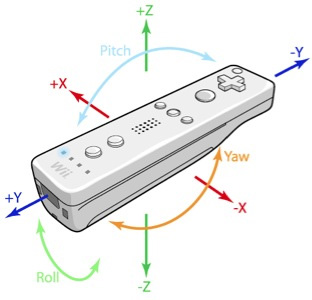
\includegraphics[width=.45\textwidth]{wiimoteAxis.png}
    \caption{\footnotesize A visual representation of the cartesian coordinate system for the Wii Remote, taken from Wii Brew\cite{wiiBrew}.}
\end{figure}

% Sette algoritmen i appendix?

The algorithm update method requires six parameters: The first three are the gyroscope's X, Y, and Z axis measurements provided in radians/, the following three are the accelerometers X Y Z in any calibrated unit. We discovered that what is defined as yaw, pitch, and roll is not universal, and which axis each corresponds to might be different for aviation and gaming controllers. Rotation about the X axis corresponds pitch, Y corresponds roll and Z corresponds to yaw such as shown in % REF TO IMAGE %WRITE MORE ABOUT HOW IT WORKS WITH ACCEL/GYRO
The algorithm returns the result as a Quaternion that need to be stored and converted to Euler angles. The formulas for converting the Quaternion to Euler angles are provided in the Madgwick paper. The formula for roll is incorrect in the paper, providing us with incorrect values, Tryggestads calculation was used for the roll conversion. The change was minor as Madgwick uses the wrong quaternion unit for roll calculation.

%SHINY PICTURZS OF OUR CODE

\section{Motea}
\label{sec:motea}
During the modification of the Motej library it soon became apparent that several parts of the library were outdated or not optimal for the current application. One problem was discovered when implementing rumbling response to alarm events. The rumble pack was turned off each time a request for status information was sent to the Wii remote. This bug was caused by the fact that Motej did not modify the status information request with the current status of the rumble pack.

It was also discovered that Motej used an outdated port to send requests to the Wii remote. Motej used the control pipe with report 0x52 to send requests. This method only works for the original Wii remotes, and will not work for the newer models. During testing the original Wii remote with external MotionPlus was used and therefore this problem was not discovered before later in the development phase.

Because of all the small bugs and the large portions of the library that were not used it was decided to create a lightweight Wii remote library from scratch. The new library was based on the general structure of Motej, and some of the code was also reused. Motea uses the data pipe for both sending and receiving data from the Wii remote. This way the new library should suppor the newer Wii remotes. 

Currently these input report modes are supported:
\begin{description}
	\item[0x20] Status information
	\item[0x21] Read memory and registers
	\item[0x37] Core buttons, acceleromter, extension data (gyroscope)
\end{description}

Report mode 0x37 also contains bytes with data from the IR camera, but this functionality was not needed and therefore not added to the Motea library.

Supported output reports are:
\begin{description}
	\item[0x11] Set LEDs and activate rumble pack
	\item[0x12] Sed data report mode (only 0x37 will be used)
	\item[0x15] Status information request
	\item[0x16] Write to memory and registers (used for activating MotionPlus)
	\item[0x17] Read memory and registers (for calibration reports)
\end{description}

The new library has working support for rumbling and connecting the MotionPlus extension while rumbling, which also was problematic with Motej. Motea also sends requests for status information and checks for MotionPlus (if not connected) each second. This way any class listening to status information events get regular updates, and not just when an extension is connected.

\section{Prototype application}
The graphical user interface of the application is quite simplistic, there are two reasons for this. The first being that this prototype is more focused on the technology and viability of a bio-feedback system based on a Wii Remote and an Android device, then the user interface. The application is intended those who do not have great coordination or muscle control, so we are trying to keep the interaction with the phone to a minimum, and when they do need to interact with it, then it should be easy and very simple.

The GUI consists of 3 components, two buttons and a visual representation of the Wii Remote. A connection with the Wii Remote is attained by pressing the (1) and (2) buttons on the Wii Remote, and afterwards pressing the "Connect" button on the application. The button will change from "Connect" to "Connecting.." in order to inform the user that it is attempting to establish a connection. Once a connection has been established the "Connect" button will be grayed out an changed to "Connected". A connection is confirmed by the 3D box coming to life, and any movement of the Wii Remote is mirrored by the box on screen. A successful connection will also be indicated on the Wii Remote due to the LEDs on the controller being lit. The LEDs represent the battery life; All four LEDs lit means that the Wii Remote battery is full.

PICTURE OF APPLICATION

Once a successful connection has been established the Wii Remote should be calibrated in order to achieve optimal accuracy. Through the use of the gyro data the Madgwick algorithm is able to correct inaccurate data. The WiiMote does contain calibration constants sadly these are not accurate. A gyro velocity of up to 30 rad/s is reported when the WiiMote is in fact standing still. Through manual calibration this error is reduced to approximately 0. Calibration is achieved by placing the Wii Remote in the desired position and then pressing the "Calibrate" button.

The position of the WiiMote at the time of calibration will be set as the starting point when calculating angular displacement. Once the angular displacement is above the set threshold a beep sound will be activated in set internvals, and the WiiMote will vibrate in tune with the beeps. The frequency of the vibration and beeps will increase as the angular displacement increases, and 90 degrees being the max intensity.

\chapter{Viability Testing}
The following chapter presents factors we believe to be of relevance and important to test so that the viability of the system can be established. The initial section will describe what factors are to be tested, why these are being tested, and what we find acceptable parameters to be. The later section describe the tests performed in order to test each factor and the attained results. All the tests are performed using a Galaxy Nexus \cite{galaxyNexus} and a Wii Remote with a Motion Plus extension unless stated otherwise.

\section{Deciding factors}
The first factor that came to mind was battery life. How was the battery life on the Wii Remote and on the Android smartphone. The majority of Android devices come with specific batteries which are easily rechargeable and have a well documented battery life according to the use. The Wii Remote on the other hand does not. If the battery life is too short it can be cumbersome to change them, come with increase cost and reduce overall satisfaction with the system. We estimated that a Android device battery would at least last 24 hours and be charged while the user is asleep and hence the same rules should apply to the Wii Remote. Therefore a minimum parameter of 24 hours was set in order for the battery life to be satisfactory.

Range is something that should always be considered when dealing with wireless devices. It might be desirable for a user to not carry his phone around if he is at home, or work. Having an awareness of the range would allows the user to comfortably walk around without having to worry about keeping close to the device at all times. Most manufacturers use the Bluetooth Class 2 microchip which allows a minimum range of 10 meters, and thus this is what we consider to be the acceptable value.

The performance of the application on the smartphone needed also to be tested. This was done to ensure that application was smooth and no unexpected behavior would occur on various devices. We found this factor satisfactory if we noticed no hitches or lag from the application in addition that all the functions worked as intended.

We found it necessary to test the initial functionality and tactile feedback that the system provided. The tests were of a qualitative nature and we wanted to see if there were any immediate issues we discovered with the system that could be rectified. We did not perform any major tweaking or spend a large amount of resources finding the optimal position and threshold settings for the system. 

\section{Battery life}
The WiiMote is powered by two AA batteries and battery life is based on several factors. The official response from Nintendo is "up to 30 hours" \cite{wiiBattery}

As the prototype application does not utilize all of the features the Wii Remote offers but only the sensor data and rumble feature we hope to have a battery life of at least 30 hours wit ha fresh set of batteries. The batteries used to perform the test are a fresh set of Duracell Ultra Power batteries. These were chosen because they are available from almost any convenient store. The Galaxy Nexus was connected to power during the entire time, while the WiiMote had a fresh set of batteries put into it before each test.

The application used was a slightly modified version of our prototype application. The changes should have no unintended impact of the battery life of the Wii Remote as most of them were computational and interface data on the Android device, which is not being tested. A timer was added that starts counting when a WiiMote is connected, and stops when the connection is lost. The threshold alarm was disabled, and instead a button allowing manual enabling and disabling of rumbling was added.

Two set of tests were performed in order to measure battery life. The first set involved the WiiMote transmitting sensor data to the Galaxy Nexus. The second test set had the WiiMote rumbling while sensor data was being transmitted. Time and resource constraints limited what type of battery tests could be performed, so two extremes was decided as a good indicator of expected battery life. The results from the tests can be seen in %REFERENCE TO FIGURE

\begin{table}[h]
\centering
\setlength{\extrarowheight}{0,2cm}
\begin{tabular}{p{2cm}|p{4.75cm}|p{4.75cm}|}
\cline{2-3}
&\multicolumn{2}{c|}{\textbf{Time}}\\ \hline
\textbf{Test Nr.} &\textbf{No Rumble} & \textbf{Rumble} \\ \hline
1 & 63:18:04 & 33:12:44 \\ \hline
2 & 61:56:21 & 33:13:45 \\ \hline
3 & 62:23:55 & 33:10:28 \\ \hline
\end{tabular}
\caption{There seemed to be no great variation in the test data, so after 3 runs we concluded that the data was consistent enough.}
\label{}
\end{table}

The table shows a consistent time of around 33 hours with constant rumble and approximately 62 when only sensor data is being transmitted. Our system will have a mix of both depending on the amount of feedback it needs to provide. The expected uptime on the battery type we tested is then somewhere between 33 - 62 hours of use. Considering constant rumbling is highly unlikely, we assume that the battery life is on higher end of the scale.

Our initial expectation was a minimum of 24 hours, the results were far beyond what we expected it to be, which speaks positively for the Wii Remote as possible sensory device. We used brand batteries that boast about longer battery life, but with such a high numbers we believe that even a non-brand and rechargeable battery will be above the 24 hour minimum limit.
\section{Range}
The connection was tested with a 30 meter distance in a open landscape computer lab and no connection issues were present. With a room in between the WiiMote and Android device a range of 15 meters was reached before signs of signal loss started to appear, by this we mean that the 3D object was not updating smoothly or the WiiMote started vibrating franticly.

A distance of 30 meters in an open landscape and 15 meters between walls is well beyond our initial expectation of 10 meters and helps establish the Wii Remote as a viable sensory device for our system.
\section{Performance}
A performance test was performed with the identical software version across three different Android devices. The three device were: A stock HTC One V, stock Google Nexus and a HTC Desire HD using Cynaogenmod 7. The test consisted of connecting the Wii Remote, calibrating, and then changing the orientation of the Wii Remote in several directions at increasing speeds.

\subsection{HTC One S}
As mentioned in the Limitations (ADD REF!?) section our understanding was that the Wii Remote would not be able to establish a connection with an Android device that has HTC Sense on it. The device performed satisfactory within reason, when orientation changed rapidly and franticly it started to shows signs of not being able to keep up with all the rapid alterations.

\subsection{Google Nexus}
The google nexus is considered to be a stock developer phone with no modifications from the re-seller. Surprisingly this one performed the worst out of the test group. At higher speeds stutter became apparent and the sound and vibration started too lag, in addition to the cube not updating. The program would freeze and lag for a second and in the next two seconds it would try to make up for the lost feedback by increasing the frequency of sound and vibration.

\subsection{HTC Desire HD}
This is the oldest model out of the three devices. Like the HTC one S it presented issues with not being able to keep up with the orientation change and reflect it properly in the frequency of the audio and vibration.

\subsection{Performance results}
The fact that the application worked on an Android device with HTC Sense was a major surprise for us, this might mean that devices with Android version 3.0 and 4.0 from HTC do support reflection and allow the application to function properly on the system. The issues that became apparent with the sound and vibration stems from our implementation of the functionality. We focused on getting the intended, and not optimizing performance, we believe that with some time given to optimize this issue can be resolved.

\section{Threshold alarm}
Testing of the threshold alarm were conduced with the writers of this paper as the only test subjects.

A problem we discovered was that the WiiMote vibration was not strong enough for the user to notice that it was vibrating. During the low frequency pulsing vibrations it was nearly impossible to notice the vibrations unless the user was aware it was about to happen. At higher frequency it was slightly better, but still not satisfactory. During the test the WiiMote was facing with the button surface away from the body. The batteries inside the WiiMote are quite large and heavy and we noticed they were soaking most of the vibration and the area around the batteries was barely vibrating. Turning the WiiMote to  so that the surface containing buttons was facing inwards gave slightly better results. We attempted to remove the strap and hold the WiiMote manually against the skin. This did improve the results but did not seem feasible in a real uncontrollable environment.
\chapter{Final thoughts}

\section{Discussion}

\subsection{RQ1}
Making the source code reusable for further development was an important, and modifiability was therefore one of the main focuses when designing the software architecture. Event-driven architecture was used to to achieve loose coupling between the different components. This gives us the option to replace the Wii remote with other types of sensors without major changes to the rest of the code. A handler class for the Wii remote was added to make it easier to implement support for multiple Wii remotes at a later date. This class also helps separate the Wii remote components from the rest of the system.processing sensory data in fall detection and prevention applications.

\subsection{RQ2}
Initially two different game controllers were considered as possible sensors; these controllers were the Playstation Move and Wii remote respectively. The PS Move Controller was the superior in respect to the sensors, with built in magnetometer and gyroscope. However, it soon became apparent that this controller was not a viable option. This was due to the lack of documentation on the reverse engineering of this controller, as well as the fact that there only exists one API. The reverse engineering of the Wii remote on the other hand is well documented through multiple communities and a multitude of APIs in different languages. The focus of the project therefore shifted toward supporting the Wii Remote.

There were several Wii remote libraries written in Java, where Motej was considered the most complete. There was some concern about the fact that all of these Java based libraries were at least three years old, including Motej. Though Motej was helpful as base for the overall structure as well as a good learning tool for understanding the reverse engineering of the Wii remote, during the development phase it became apparent how outdated the library actually was. This is why we eventually decided to write our own lightweight library called Motea. One of the reasons for choosing the Wii remote was the many Java libraries that existed. The amount of work put into modifying Motej and creating Motea was much greater than expected. In retrospect, the Playstation Move might have been a viable option.

\subsection{RQ3}
The prototype developed in this project as well as other applications CITATIONNEEDED have shown that modern smartphones are more than powerful enough to function as a hub for processing sensory data in fall detection and prevention applications. In our project we wanted to explore the possibility of using cheap, off-the-shelf motion based game controllers as the external sensors for the system. 

Madgwick’s AHRS algorithm was used to calculate the orientation of the Wii remote. The algorithm is run on every sensor event, approximately ten times per second. Modern smartphones have no problem doing these calculations in real-time, while also rendering the 3D-cube. 

The limitations of the system is the lack of support for reflection used to access the L2CAP Bluetooth protocol which is required by the Wii remote. Initial research led us to believe that HTC and Samsung devices running stock ROMs would not support accessing L2CAP through reflection, and thus leave the application unable to connect to the Wii remote. To our surprise the application work fine on the HTC One S during the testing phase. HTC phones running version 4 of the Android OS might therefore be supported, though this has not been investigated further. Having an application that works out of the box on a major smartphone brand is an important for the viability of such an application.

\subsection{RQ4}
The viability tests were primarily positive and exceeded the minimum parameters we had set for our system. The Battery life was a positive surprise, the life expectancy was beyond our minimum 24 hours and the ``up to 30 hours stated by Nintendo. Seeing as constant rumble provided 33 hours and no rumble at all gave around 62 it is safe to expect that our application will be above 40 hours as users of the application will ideally make the vibration stop as soon as they can sense it. 

The Wii remote was connected to the smartphone using the robust and well proven Bluetooth technology for continuous streaming of sensory data. The Class 2 Bluetooth radio used in smartphones and motion controllers gives a theoretical range of 10 meters. Our tests indicates that the actual range is even greater than this. A range of more than 10 meters should be more than satisfactory considering the use of the application.

The feedback test showed that detecting the vibration might be a problem. The vibration provided by the Wii Remote was barely noticeable through the belt used for attachment to the user. This might be due to the heavy battery absorbing the vibration or the rumble engine simply not being powerful enough. It was necessary to press the Wii Remote firmly against the body before the vibration could be clearly felt. The audio feedback worked as intended and was easy to interpret. The implementation of the sound alarm needs further work and testing to assure that it work smoothly on all versions of the Android OS.

\subsection{Threats to validity}
One possible threat to validity is the software architectures focus on modifiability. As a proof-of-concept prototype system, prone to constant changes in hardware and functionality, a highly modifiable architecture is essential. For a system with specifed hardware and functionality modifiability would not be as crucial. In such a system availability and performance would be more important. For a fall detection/prevention application to be used in practice both high availability and performance would have to be guaranteed for obvious reasons. The architectural choices presented in this paper is therfore to be seen from a prototyping point of view, and not a system for production.

The viability tests did posses a large sample size or were performed in a highly controlled environment. The small sample size prevents us from strengthening our conclusions with statistical data or generalize our findings. Therefore the conclusions we come to in this paper are limited to our implementation or a similar mobile biofeedback system. If our system is viable or not is based on knowledge gained through research and working on the paper. However this is not close to the knowledge possessed by experts in the field, and review by such an individual might come to a different conclusion.


\section{Conclusion}

\textit{What architectural decision should be considered in a mobile biofeedback system?}


We created a software architecture with focus on modifiability and usability. Modifiability was important to ensure that different components, e.g. sensor choice, could be replaced or modified without effecting the system as a whole. With all the uncertainties surrounding sensor choice and functionality being able to change different components quickly is paramount. Though little effort was put into the graphical user interface in this project, usability was important for the prototype code to be reused in future work. The Model-View-Controller pattern was used to separate the GUI components, this in combination with the many features offered by the Android OS, creating a GUI at a later date should not be challenging.

\textit{Which game controllers are viable options in the creation of a mobile biofeedback system?}


There was no proper documentation on reverse engineering or Java based libraries for the PS Move Controller. The Wii Remote reverse engineering had been well documented by the community and several Java based libraries existed. Eventually it was discovered that all of the libraries were simply too old and inefficient to be of real use, and therefore we have created our own light-weight library under the name Motea.

\textit{What are the limitations of using the Android OS and game controllers in the creation of a biofeedback system?}


Older smartphones running stock firmware from major Android brands such as HTC and Samsung cannot run the application due to the lack of support for Bluetooth L2CAP protocol. It was discovered that an HTC smartphone running version 4.0 of the stock firmware was able to run the application however. This probably means that newer HTC phones can run the application out of the box, though this was not tested further.


\textit{What are important factors that will determine if the system has any viability as a mobile bio-feedback system, and what are acceptable parameters for these factors?}


We concluded that the most important factors for an initial prototype was battery life, range, performance, and investigating if the audio and vibration feedback is good enough. The three factors were all beyond satisfactory with a battery life of 60 hours, a range of 30 meters and a smooth performance proved that the prototype is viable. The vibration feedback was not satisfactory and was perceived as too weak to be noticeable, but the audio worked well.

\section{Further work}
This project have shown that Android smartphones with the correct software can connect and receive sensor data form Wii remotes. Our viability testing have shown that both battery life and range is satisfactory. Still, there is a lot of work to be done to create a functioning fall detection/prevention system using Android smartphones and Wii Remotes. First, the application needs to provide helpful feedback reducing the risk of falls, and alerting about falls. Second, the architecture needs to be tested in respect to availability and performance. Third, a user friendly user interface has to be created in order to allow older people, often unexperienced with modern technology, to use the application efficiently and safely. Fourth, an experiment has to be conducted to evaluate the effectiveness of the system and establish the best number of sensors and their optimal position.
\begin{comment}
+ Only an initial prototype
+ Optimization
+ Create proper algorithms for the threshold, and tweak sensor values
+ A more user friendly interface
+ Experiment with multiple controllers or different sensors ?
\end{comment}

\bibliographystyle{plain}
\bibliography{references}
\appendix

\chapter{Output Reports}
\label{app:outputReports}
Motea sets the report mode to 0x35 as soon as the connection to the Wii remote is established. This is done by sending the following bytes to the Wii remote:
\begin{quote}
0xA2 0x12 0x04 0x35
\end{quote}
The first byte indicates that it is an output report, the second byte is the ID of the report type, the third byte indicates whether to use continuous reporting (send report even when there has been no change to the data) and the fourth indicates which report mode to set. The report mode has to be set again whenever an extension is discovered, this can be detected by the fact that you receive a status information report without requesting one. In such cases Motea immediately sends a request to set the report mode to 0x35.

Report mode 0x35 contains core button (0xbb), acceleromter (0xaa), and extension data (0xee):
\begin{quote}
0xA1 0x35 0xbb 0xbb 0xaa 0xaa 0xaa 0xee 0xee 0xee 0xee ... (16 bytes of type 0xee)
\end{quote}

The LEDs on the Wii remote can be controlled by using output report 0x11:
\begin{quote}
0xA2 0x11 0x80
\end{quote}
The third byte indicates which lights to turn on, the four most significant bits of this byte each represents one LED (in the example above the rightmost byte is enabled):
\begin{quote}
0b0000 0000 : no lights\\
0b1000 0000 : rightmost LED enabled\\
0b1100 0000 : the two rightmost LEDs enabled\\
etc.
\end{quote}
Motea also uses this report mode to initialize the rumble pack. The least significant bit of the third byte of any output report turns sets the status of the rumble pack, where 1 is on and 0 is off. As an example, let us say we have the two rightmost LEDs activated and the rumble pack is to be turned on, the report would look like this:
\begin{quote}	
0xA2 0x11 0xC1\\
(0xC1 = 0b1100 0001 the least significant bit representing the rumble pack)
\end{quote}
As previously stated all output reports have to change the least significant bit of the third byte to one if the rumble pack is to stay active. Therefore Motea has to keep track of the state of the rumble pack and change the output reports accordingly. All examples in this section, other than the one above, will assume that rumbling is turned off.

Status information can be requested by sending:
\begin{quote}
0xA2 0x15 0x00
\end{quote}
A status information report with ID 0x20 is then sent from the Wii remote to the host:
\begin{quote}
0xA1 0x20 0xbb 0xbb 0xss 0x00 0x00 0xll
\end{quote}
0xbb (bytes 3 and 4) contains data about the core buttons. 0xss contains data about which LEDs are enabled and whether the following features are enabled: speaker, extension controller, and continouous reporting. 0xll holds the battery level. 

Writing to registers is done by sending:
\begin{quote}
0xA2 0x16 0x04 0xaa 0xaa 0xaa 0xll 0xdd 0xdd ...
\end{quote}
Here 0xaa (bytes 4-6) represents the register address to write to. 0xll is the number of bytes to write. 0xdd (bytes 8-) is the data to be written to the register, usually only one byte is written.

Reading from registers/memory is done by sending:
\begin{quote}
0xA2 0x17 0xmm 0xaa 0xaa 0xaa 0xll 0xll
\end{quote}
0xmm sets whether to read from memory or from the registers, in motea only the calibration report for the accelerometer is read from memory. 0xaa (bytes 4-6) is the address to read from. 0xll (bytes 7 and 8) is the length of data to be read. After a read request is sendt the Wii remote sends the data in return using a report with ID 0x21:
\begin{quote}
0xA1 0x21 0xbb 0xbb 0xse 0xaa 0xaa 0xdd 0xdd ... (16 bytes of the type 0xdd)
\end{quote}
0xb (byte 3-4) is core button data. 0xse holds both the size of the data returned and the error flag. 0xdd (bytes 8-23) contain the requested data (as long as there was no error).

\chapter{MotionPlus}
\label{app:gyroParse}

When you plug in a normal extension to the Wii remote it is automatically receive a status information report notifying that an extension has been connected. Pluging in the MotionPlus however, will not result in such a status information report. To check if the MotionPlus extension is pluged in, the two bytes from Wii remote register address 0xA600FE has to be read by sending the read request:
\begin{quote}
0xA2 0x17 0x04 0xA6 0x00 0xFE 0x00 0x02
\end{quote}
After sending this request a data report with ID 0x21 is sent in return containing the requested data. The received data report contains the two bytes read from register 0xA600FE. The meaning of these bytes are shown in table~\ref{tab:motionPlusStatus}. If the MotionPlus extension is not connected the data report will fail with error 7.
\begin{table}[h!]
\begin{tabularx}{\textwidth}{|l|X|}
\hline
Value  & Meaning \\ \hline
0x0005 & MotionPlus is pluged in, but not initialized \\ \hline
0x0405 & No longer active MotionPlus\\ 
\hline
\end{tabularx}
\caption{\footnotesize MotionPlus status}
\label{tab:motionPlusStatus}
\end{table}

After confirming that the MotionPlus extension is pluged in, the next thing to do is to initialize it. This is done by writing 0x55 to 0xA600F0, by sending the following report:
\begin{quote}
0xA2 0x16 0x04 0xA6 0x00 0xF0 0x01 0x55
\end{quote}

When the MotionPlus has been initialized it has to be activated before we can receive data from it. This is done by writing 0x04 to register address 0xA6 0x00 0xFE:
\begin{quote}
0xA2 0x16 0x04 0xA6 0x00 0xFE 0x01 0x04
\end{quote}
After the MotionPlus extension has been activated the Wii remote will send a status information report, informing that an extension has been connected. Now the extension bytes of data report 0x35 will contain gyroscope data form the MotionPlus.

The 32 bytes from register 0xA60020 holds the calibration data for the MotionPlus. According to the WiiBrew wiki \cite{wiiBrew} it is still unclear how they work. However, by looking at the WiiMoteLib \cite{wiiMoteLib} library an implementation using this calibration data was found. Unfortunately this implementation is not very accurate, at least not compared to manual calibration. Aquireing the data is done by sending the read request:
\begin{quote}
0xA2 0x17 0x04 0xA6 0x00 0x20 0x00 0x32
\end{quote}

Extension data is received with every report of ID 0x35:
\begin{quote}
0xA1 0x35 0xbb 0xbb 0xaa 0xaa 0xaa 0xee 0xee 0xee 0xee ... (16 bytes of type 0xee)
\end{quote}
Here 0xbb represents core button data and 0xaa represents acceleration data. The extension data is contained in the 16 last bytes shown by 0xee above. The gyroscope data is contained in the 6 first bytes of the extension data. The data format is shown in figure~\ref{fig:motionPlusDataFormat}. The gyroscope has two modes: fast and slow. These values tells us what type of scaling to use to get the correct degrees per second. According to WiiBrew \cite{wiiBrew} 20 units correspond to 1.45 deg/s in slow mode and 6.59 deg/s in fast mode. Motea uses slightly different values, taken from WiiMoteLib \cite{wiiMoteLib}: 20 units corresponding to 1 deg/s in slow mode and 5 deg/s in fast mode. Which of these values give more accurate data has not been tested, and since the Madgwick algorithm \cite{madgwick} compensates roll and pitch error using the acceleromter, a small error in the gyroscope data can be tolerated. 
\begin{figure}[h!]
  \centering
    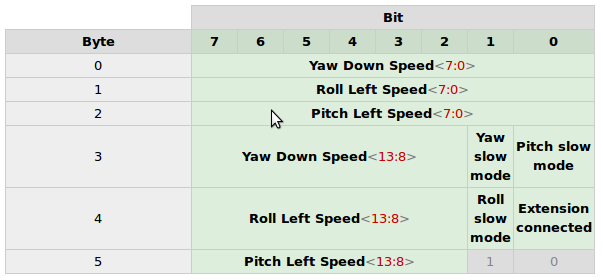
\includegraphics[width=.80\textwidth]{motionPlusDataFormat.png}
    \caption{\footnotesize Motion Plus data gyroscope data format}
    \label{fig:motionPlusDataFormat}
\end{figure}

Motea parsing and calibrating gyroscope data:
\begin{lstlisting}
// Get fast/slow mode
boolean yawFast = ((extensionData[3] & 0x02) >> 1) == 0;
boolean rollFast = ((extensionData[4] & 0x02) >> 1) == 0;
boolean pitchFast = ((extensionData[3] & 0x01) >> 0) == 0;

// Get raw data
float yaw = 
	((extensionData[0] & 0xff) | ((extensionData[3] & 0xfc) << 6));
float roll = 
	((extensionData[1] & 0xff) | ((extensionData[4] & 0xfc) << 6));
float pitch = 
	((extensionData[2] & 0xff) | ((extensionData[5] & 0xfc) << 6));

// Manual calibration
if (!calibration.isFinished()) {
	calibration.addCalibrationData(yaw, roll, pitch);
	if (calibration.isFinished()) {
		calibrationData = calibration.getCalibratedData();
	}
}

// Calibrate raw data
yaw -= calibrationData.getYaw0();
roll -= calibrationData.getRoll0();
pitch -= calibrationData.getPitch0();

// Set scaling
if (yawFast) {
	yaw /= HIGHSPEED_SCALING;
} else {
	yaw /= LOWSPEED_SCALING;
}

if (rollFast) {
	roll /= HIGHSPEED_SCALING;
} else {
	roll /= LOWSPEED_SCALING;
}

if (pitchFast) {
	pitch /= HIGHSPEED_SCALING;
} else {
	pitch /= LOWSPEED_SCALING;
}
\end{lstlisting}

\end{document}
